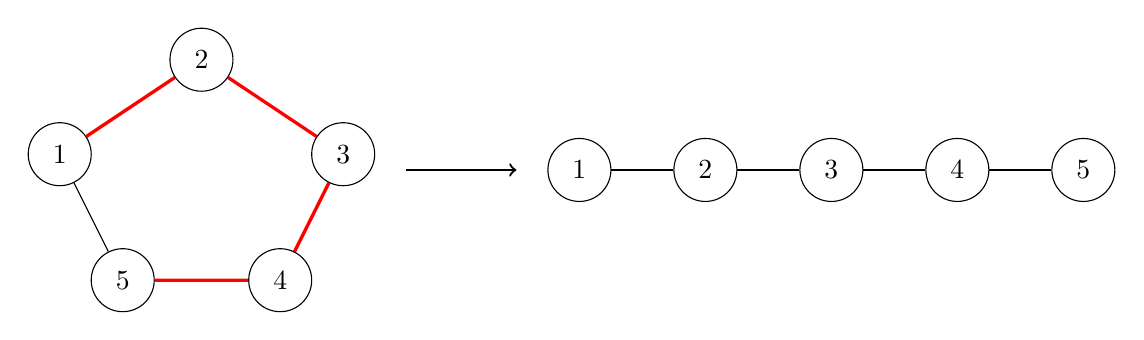
\begin{tikzpicture}[
    vertex/.style={circle, draw, minimum size=8mm, inner sep=0pt},
    edge/.style={-},
    pathedge/.style={-, very thick, red},
    trans/.style={->, thick}
]
    % Grafo 1: ciclo de 5 vértices em forma de pentágono, maior espaçamento
    \node[vertex] (a1) at (0,2) {1};
    \node[vertex] (b1) at (1.8,3.2) {2};
    \node[vertex] (c1) at (3.6,2) {3};
    \node[vertex] (d1) at (2.8,0.4) {4};
    \node[vertex] (e1) at (0.8,0.4) {5};
    
    % Arestas do ciclo
    \draw[edge] (a1) -- (b1);
    \draw[edge] (b1) -- (c1);
    \draw[edge] (c1) -- (d1);
    \draw[edge] (d1) -- (e1);
    \draw[edge] (e1) -- (a1);
    
    % Caminho hamiltoniano destacado em vermelho
    \draw[pathedge] (a1) -- (b1) -- (c1) -- (d1) -- (e1);
    
    % Seta de transformação
    \draw[trans] (4.4,1.8) -- (5.8,1.8) node[midway, above]{};
    
    % Grafo 2: caminho em linha com maior espaçamento
    \node[vertex] (a2) at (6.6,1.8) {1};
    \node[vertex] (b2) at (8.2,1.8) {2};
    \node[vertex] (c2) at (9.8,1.8) {3};
    \node[vertex] (d2) at (11.4,1.8) {4};
    \node[vertex] (e2) at (13.0,1.8) {5};
    
    \draw[edge] (a2) -- (b2) -- (c2) -- (d2) -- (e2);

\end{tikzpicture}